\section{CƠ SỞ LÝ THUYẾT}\label{sec:co_so_ly_thuyet}

Chương này trình bày các nền tảng lý thuyết được dùng trực tiếp trong mô hình: kiến trúc mạng Campus truyền thống (phân cấp, VLAN, dự phòng, định tuyến, dịch vụ, tường lửa) và hai công nghệ điều khiển bằng phần mềm SDN, SD-WAN, rồi khảo sát các nghiên cứu liên quan để xác định vị trí của đề tài.

\subsection{Mạng Campus và mô hình phân cấp}

Mạng Campus là mạng nội bộ trong phạm vi một khuôn viên như trường đại học, kết nối khoa, phòng ban, phòng máy, thư viện và hệ thống máy chủ. Khi trường có nhiều cơ sở, bài toán mở rộng thành mạng đa cơ sở (multi-site): ngoài LAN của từng cơ sở còn cần hạ tầng WAN để cơ sở phụ dùng các dịch vụ đặt tại cơ sở chính. Mạng Campus hiện đại phải đáp ứng năm yêu cầu: hiệu năng, tính sẵn sàng (không có điểm lỗi đơn tại gateway, lõi, tường lửa, WAN), phân đoạn và bảo mật, quản trị tập trung, khả năng mở rộng.

Mô hình Core--Distribution--Access (Hình~\ref{fig:core_distribution_access}) chia mạng thành các tầng có chức năng rõ ràng, giúp thiết kế, vận hành và giới hạn phạm vi ảnh hưởng của sự cố. Tầng Access kết nối thiết bị đầu cuối, gán VLAN cho cổng. Tầng Distribution tập trung đường lên từ Access và là điểm đặt cơ chế dự phòng; với mạng quy mô vừa, định tuyến liên VLAN có thể dồn lên Core (\textit{collapsed core}). Tầng Core là xương sống chuyển tiếp tốc độ cao và nối ra biên mạng, cần đơn giản và có dự phòng. Trong đề tài, cơ sở chính dùng đủ ba tầng; các cơ sở phụ quy mô nhỏ dùng mô hình rút gọn, trong đó tường lửa chi nhánh kiêm lõi định tuyến (\textit{Firewall-as-Core}).

\begin{figure}[H]
    \centering
    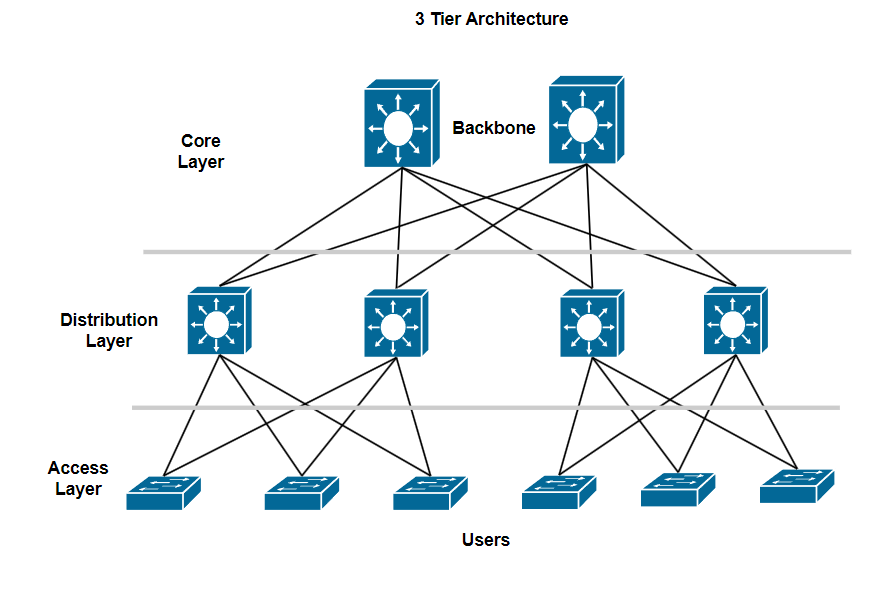
\includegraphics[width=0.78\textwidth]{image/mohinh.png}
    \caption{Mô hình mạng phân cấp Core--Distribution--Access}
    \label{fig:core_distribution_access}
\end{figure}

\subsection{VLAN, trunk 802.1Q và định tuyến liên VLAN}

VLAN chia một hạ tầng switch thành nhiều mạng logic, mỗi VLAN là một miền quảng bá riêng. Cổng access thuộc một VLAN và không gắn thẻ; cổng trunk mang nhiều VLAN, chuẩn IEEE 802.1Q \citep{ieee8021q_2018} chèn thẻ 4 byte gồm TPID \texttt{0x8100} và VLAN ID 12 bit. Danh sách VLAN được phép trên trunk cần giới hạn đúng nhu cầu để thu hẹp miền quảng bá. Giao tiếp giữa các VLAN cần định tuyến: dùng SVI trên switch lớp 3 (cách dùng trên Core-SW1/2) hoặc \textit{router-on-a-stick} với sub-interface 802.1Q (cách dùng trên tường lửa chi nhánh). Khi lưu lượng liên VLAN bắt buộc qua gateway, nó có thể được kiểm soát bằng ACL, tường lửa hoặc chính sách của Controller.

\subsection{Cơ chế dự phòng lớp 2 và lớp 3}

STP và Rapid-PVST+. Kết nối dự phòng tạo vòng lặp lớp 2; vì frame Ethernet không có TTL, broadcast lặp vô hạn gây \textit{broadcast storm} và \textit{MAC flapping}. STP (IEEE 802.1D \citep{ieee8021d_2004}) bầu Root Bridge và chặn cổng dư để tạo cây không vòng; RSTP (IEEE 802.1w) rút thời gian hội tụ từ 30--50 giây xuống vài giây; Rapid-PVST+ chạy một tiến trình RSTP cho mỗi VLAN. STP chỉ hoạt động trên thiết bị trao đổi BPDU: khi một phần mạng do SDN Controller điều khiển và tắt STP (như OVS trong đề tài), Controller phải tự tính cây và chặn cạnh dư.

EtherChannel và LACP. EtherChannel gộp nhiều liên kết song song thành một Port-Channel có băng thông bằng tổng thành viên, STP xem như một cổng và vẫn chạy khi một thành viên lỗi. LACP (IEEE 802.3ad, nay thuộc IEEE 802.1AX \citep{ieee8021ax_2020}) là giao thức thương lượng theo chuẩn mở.

VRRP. Máy trạm chỉ khai một default gateway nên gateway hỏng làm cả VLAN mất kết nối. VRRP (RFC~5798 \citep{rfc5798_vrrpv3}) cho nhiều router chia sẻ một địa chỉ IP ảo; router có priority cao nhất là \textit{Master}, trả lời ARP bằng MAC ảo \texttt{0000.5e00.01xx}; khi Master ngừng quảng bá quá \textit{Master Down Interval}, \textit{Backup} tiếp quản mà máy trạm không phải đổi cấu hình.

\subsection{Định tuyến}

Thiết bị chọn tuyến theo \textit{longest prefix match}, rồi khoảng cách quản trị và metric; nhiều tuyến cùng metric có thể dùng song song (ECMP).

OSPF (RFC~2328 \citep{rfc2328_ospfv2}) là giao thức trạng thái liên kết: router trao đổi LSA để có cùng cơ sở dữ liệu topology trong một area rồi chạy Dijkstra tìm đường ngắn nhất; láng giềng ở trạng thái \texttt{FULL} khi đã đồng bộ; \texttt{default-information originate} quảng bá tuyến mặc định vào miền OSPF. Trong đề tài, OSPF Area~0 chạy giữa hai Core, tường lửa biên và hai vEdge của cơ sở chính.

BGP (RFC~4271 \citep{rfc4271_bgp4}) định tuyến giữa các AS, chạy trên TCP 179 và chọn tuyến theo tập thuộc tính (AS\_PATH, NEXT\_HOP, LOCAL\_PREF\ldots), phù hợp thể hiện chính sách giữa khách hàng và nhà cung cấp; nhà cung cấp thường gửi tuyến mặc định cho khách hàng bằng \texttt{default-originate}. Đề tài dùng eBGP làm underlay của hai nhà cung cấp Internet và MPLS.

Tuyến tĩnh có theo dõi. Hai tuyến mặc định với khoảng cách quản trị khác nhau tạo \textit{floating static route}: tuyến dự phòng chỉ dùng khi tuyến chính biến mất. Vì tuyến tĩnh chỉ mất khi cổng ra down, cơ chế IP SLA (trên ASA là \texttt{sla monitor}) định kỳ ping một đích tham chiếu; đối tượng \texttt{track} gỡ tuyến chính khi đích không phản hồi để tuyến dự phòng được kích hoạt.

\subsection{Dịch vụ mạng nền tảng}

DHCP \citep{rfc2131_dhcp} cấp địa chỉ, gateway, DNS và tên miền qua bốn bản tin DORA. Vì DISCOVER là broadcast, khi máy chủ nằm ở VLAN khác thì gateway phải chạy \textit{DHCP Relay} (\texttt{ip helper-address}): relay chuyển bản tin thành unicast và ghi địa chỉ giao diện vào \texttt{giaddr} để máy chủ chọn đúng scope. Ở chi nhánh nhỏ, DHCP thường chạy ngay trên gateway để vẫn cấp địa chỉ khi WAN gián đoạn.

DNS \citep{rfc1035_dns} phân giải tên thành địa chỉ; máy chủ nội bộ quản lý zone thuận (A, MX) và zone ngược (PTR). Hậu tố \texttt{.local} được RFC~6762 \citep{rfc6762_mdns} dành cho Multicast DNS nên nhiều hệ điều hành không hỏi máy chủ DNS cho \texttt{*.local}; từ năm 2024, ICANN dành riêng hậu tố \texttt{.internal} cho mạng riêng.

Syslog, Web, Mail. Syslog (UDP 514, RFC~5424 \citep{rfc5424_syslog}) tập trung nhật ký từ thiết bị về một máy chủ. Web hiện đại chạy HTTPS, chứng chỉ phải chứa đúng tên miền trong trường SAN. Mail gồm SMTP (TCP 25) giữa máy chủ, Submission (TCP 587, có xác thực) và IMAP (TCP 143/993); bản ghi MX chỉ định máy chủ nhận thư.

\subsection{Tường lửa trạng thái và DMZ}

Tường lửa trạng thái ghi nhớ từng phiên trong bảng kết nối và tự cho phép lưu lượng phản hồi của phiên hợp lệ. Trên Cisco ASA, mỗi giao diện có \texttt{nameif} và \texttt{security-level} 0--100: lưu lượng mặc định đi từ mức cao sang mức thấp, chiều ngược lại phải được ACL cho phép. Số phiên đồng thời còn phụ thuộc giấy phép. DMZ là vùng đặt máy chủ công bố dịch vụ (Web, Mail) với security-level trung gian: bên ngoài chỉ vào đúng cổng dịch vụ, DMZ không được tự do khởi tạo kết nối vào trong. Để loại điểm lỗi đơn tại biên, hai tường lửa chạy \textit{Active/Standby failover} \citep{cisco_asa_failover}, trao đổi trạng thái qua liên kết failover riêng; khi đơn vị Active lỗi, đơn vị Standby tiếp quản.

\subsection{Công nghệ SDN}

SDN \citep{mckeown2008openflow, kreutz2015sdn} tách mặt phẳng điều khiển khỏi mặt phẳng dữ liệu: quyết định chuyển tiếp tập trung tại Controller, switch chỉ thực thi các flow được cài xuống. Kiến trúc gồm ba lớp (Hình~\ref{fig:sdn_architecture}): lớp ứng dụng (chuyển mạch, giám sát, bảo mật) giao tiếp với Controller qua \textit{northbound API}, thường là REST; lớp điều khiển thu thập topology, thống kê và chuyển yêu cầu thành flow; lớp hạ tầng gồm các switch chuyển tiếp theo bảng flow qua \textit{southbound API}.

\begin{figure}[H]
    \centering
    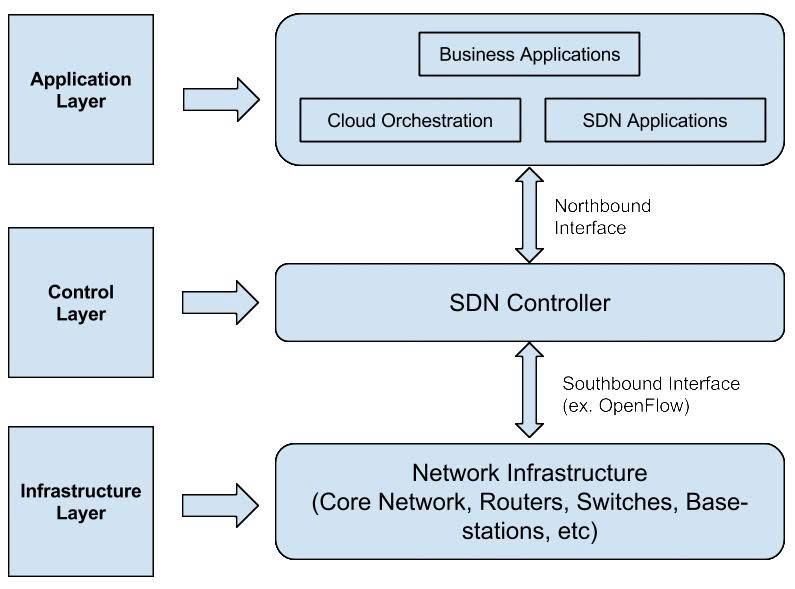
\includegraphics[width=0.64\textwidth]{image/SDN_ARCHITECTURE.jpg}
    \caption{Kiến trúc tổng quan của SDN}
    \label{fig:sdn_architecture}
\end{figure}

OpenFlow 1.3 \citep{onf_openflow_134} là giao thức southbound tiêu chuẩn, chạy trên TCP 6653. Mỗi flow entry gồm trường so khớp (cổng vào, MAC, EtherType, VLAN, IP, cổng TCP/UDP), priority, tập lệnh (output, drop, push/pop VLAN, set-field), bộ đếm, timeout và \textit{cookie}. Flow priority 0 (\textit{table-miss}) quyết định gói chưa có quy tắc, thường gửi lên Controller. Switch gửi \texttt{Packet-In}; Controller trả \texttt{Packet-Out} và/hoặc \texttt{Flow-Mod}. VLAN trong OpenFlow 1.3 được so khớp bằng trường \texttt{vlan\_vid} có bit \texttt{OFPVID\_PRESENT} (0x1000); tên \texttt{dl\_vlan} chỉ thuộc OpenFlow 1.0. Khi mất Controller, switch ở chế độ \texttt{standalone} quay về học MAC truyền thống, còn ở chế độ \texttt{secure} chỉ dùng flow đang có. Kênh điều khiển có thể đi mạng riêng (\textit{out-of-band}) hoặc chung với dữ liệu (\textit{in-band}); với in-band, một số switch tự cài quy tắc ẩn để giữ kết nối Controller, có thể gây bão broadcast nếu mạng có vòng.

OVS \citep{pfaff2015ovs, ovs_docs} là switch ảo mã nguồn mở hỗ trợ OpenFlow; mỗi bridge có DPID, phiên bản OpenFlow, địa chỉ Controller, fail mode, cổng mang \texttt{tag} (access) hoặc \texttt{trunks} (trunk). Ryu \citep{ryu_434_docs} là framework SDN viết bằng Python theo mô hình hướng sự kiện, kèm \texttt{ofctl\_rest} cung cấp REST API. ONOS \citep{onos_docs} là Controller phân tán viết bằng Java, có giao diện đồ họa và phát hiện topology qua LLDP, nhưng tốn nhiều CPU và bộ nhớ hơn Ryu.

Theo cách triển khai, SDN gồm: Open SDN (Controller điều khiển trực tiếp qua OpenFlow), SDN qua API (REST, NETCONF), SDN overlay trong trung tâm dữ liệu và Hybrid SDN (một phần mạng giữ cơ chế truyền thống \citep{vissicchio2014hybrid}). Mô hình của đề tài là Hybrid SDN: lớp 2 do Controller điều khiển, lớp 3 vẫn chạy VRRP, OSPF và STP. Ưu điểm của SDN là cái nhìn toàn cục, lập trình được và áp chính sách từ một điểm; nhược điểm là Controller trở thành thành phần trọng yếu, và khi kênh điều khiển đi chung hạ tầng dữ liệu thì phải giải quyết bài toán ``switch cần Controller để chuyển tiếp nhưng Controller chỉ tới được qua chính các switch''.

\subsection{Công nghệ SD-WAN}

SD-WAN \citep{yang2019sdwan, fu2024sdwan} áp dụng nguyên lý tách mặt phẳng điều khiển cho mạng diện rộng: tạo overlay gồm các đường hầm mã hóa chạy trên nhiều \textit{transport} (Internet, MPLS, 4G/5G) và chọn đường theo chính sách và chất lượng đo được.

Kiến trúc Cisco SD-WAN (Viptela) \citep{cisco_sdwan_design} gồm bốn thành phần: vManage (quản lý: giao diện, API, giám sát, chứng thư), vSmart (điều khiển: trung tâm OMP, phân phối tuyến, TLOC, khóa và chính sách), vBond (điều phối: điểm tiếp xúc đầu tiên, xác thực, hỗ trợ vượt NAT) và vEdge/cEdge (dữ liệu: router tại site, dựng đường hầm IPsec \citep{rfc4301_ipsec, rfc4303_esp}). Mỗi Edge có System-IP (định danh /32) và Site-ID; mọi thiết bị dùng chung \texttt{organization-name}. Edge chia bảng định tuyến thành VPN: VPN 0 cho transport và underlay, VPN 512 cho quản trị, VPN từ 1 trở lên là VPN dịch vụ chứa LAN người dùng.

TLOC, OMP, BFD. TLOC là điểm cuối đường hầm, định danh bởi (System-IP, color, encapsulation); \textit{color} (\texttt{mpls}, \texttt{biz-internet}\ldots) gán nhãn loại đường truyền. OMP \citep{cisco_sdwan_omp} chạy trong kênh DTLS/TLS giữa Edge và vSmart, mang tuyến, TLOC và thông tin dịch vụ; vSmart đóng vai trò tương tự route reflector. Mặc định các Edge dựng đường hầm full-mesh. BFD \citep{rfc5880_bfd} chạy trong mỗi đường hầm để phát hiện hỏng và đo trễ, jitter, mất gói; thời gian phát hiện bằng chu kỳ nhân hệ số, mặc định 1000~ms $\times$ 7, khoảng 7 giây.

Xác thực và chính sách. Thiết bị xác thực lẫn nhau bằng chứng thư X.509 \citep{rfc5280_x509}: Edge tạo CSR, được CA ký, cài Root CA; controller còn giữ danh sách Edge hợp lệ theo cặp chassis/serial. vSmart hỗ trợ ba nhóm chính sách tập trung áp theo \texttt{site-list}: control policy (tác động tuyến và TLOC trong OMP, ví dụ đổi \textit{preference}), AAR (định nghĩa \textit{SLA class} gồm ngưỡng mất gói, trễ, jitter và chọn đường hầm thỏa SLA cho từng lớp lưu lượng) và data policy (lọc theo 5-tuple, DSCP, prefix với hành động accept, drop, count). DIA cho Edge chi nhánh NAT lưu lượng Internet ra thẳng tại chỗ thay vì đưa về trung tâm (\textit{backhaul}), giảm tải cho cơ sở chính nhưng đòi hỏi chính sách bảo mật tại từng chi nhánh.

\subsection{Nền tảng mô phỏng EVE-NG}

EVE-NG \citep{eveng_docs} cho phép chạy đồng thời nhiều loại thiết bị: Cisco IOL, vIOS, ASAv, các thành phần SD-WAN, máy ảo Linux và Windows trên QEMU/KVM cùng máy trạm VPCS; toàn bộ topology lưu trong một tệp lab và có thể nối ra mạng thật qua giao diện Cloud. Do là môi trường ảo hóa, hiệu năng và hành vi khởi động khác thiết bị vật lý; kết quả đo phản ánh tính đúng đắn chức năng hơn là hiệu năng tuyệt đối.

\subsection{Các nghiên cứu liên quan}\label{sec:nghien_cuu_lien_quan}

SDN trong mạng Campus và doanh nghiệp. Ý tưởng điều khiển tập trung cho mạng doanh nghiệp xuất hiện từ Ethane \citep{casado2007ethane}, trong đó một controller quyết định mọi luồng theo chính sách toàn cục. OpenFlow \citep{mckeown2008openflow} được đề xuất ngay từ đầu cho mạng Campus, để nhà nghiên cứu thử nghiệm giao thức mới trên switch thật mà không ảnh hưởng lưu lượng sản xuất. Khảo sát của \citet{kreutz2015sdn} hệ thống hóa kiến trúc ba lớp, các controller và bài toán độ tin cậy của SDN. Về mặt dữ liệu, \citet{pfaff2015ovs} trình bày thiết kế của Open vSwitch, switch ảo được dùng ở tầng Distribution và Access của đề tài.

Hybrid SDN và triển khai từng phần. Chuyển toàn bộ mạng sang SDN một lần là khó trong thực tế. \citet{vissicchio2014hybrid} phân tích các mô hình kết hợp SDN với giao thức phân tán truyền thống và chỉ ra rằng mỗi mô hình có một cân bằng riêng giữa khả năng triển khai, độ bền và khả năng mở rộng. Panopticon \citep{levin2014panopticon} cho thấy chỉ cần khoảng 10\% switch tầng Distribution chạy SDN là phần lớn mạng doanh nghiệp đã vận hành như một SDN thống nhất. Khảo sát của \citet{khorsandroo2021hybrid} tổng hợp các hướng Hybrid SDN về sau. Đề tài đi theo cùng hướng này: lớp 2 do Controller điều khiển, còn tầng Core, VRRP, OSPF và tường lửa giữ cơ chế truyền thống.

Kênh điều khiển in-band và phục hồi sự cố. Khi lưu lượng điều khiển đi chung đường với lưu lượng dữ liệu, một sự cố liên kết ảnh hưởng cả hai. \citet{sharma2013inband} đo trên mạng OpenFlow in-band và kết luận rằng cơ chế phục hồi sau sự cố (restoration) không đạt ngưỡng 50~ms của mạng nhà mạng, còn cơ chế bảo vệ dựng sẵn đường dự phòng (protection) thì đạt. Kênh quản trị VLAN 99 nhiều đường của đề tài là một dạng kênh điều khiển in-band. Cây chuyển tiếp được tính lại sau khi phát hiện mất liên kết, tức là cơ chế restoration, nên thời gian gián đoạn đo được (không quá 3,6 giây) là ở mức giây chứ không phải mili giây.

SD-WAN. B4 của Google \citep{jain2013b4} là một trong những WAN điều khiển bằng phần mềm đầu tiên ở quy mô lớn, dùng điều khiển tập trung để tăng hiệu suất sử dụng đường truyền giữa các trung tâm dữ liệu. Với WAN doanh nghiệp, \citet{yang2019sdwan} mô tả kiến trúc SD-WAN, các vấn đề của WAN truyền thống (trong đó có chi phí) và các giải pháp tiêu biểu. Khảo sát của \citet{fu2024sdwan} chia nghiên cứu SD-WAN thành bốn hướng: kỹ thuật lưu lượng, tối ưu mạng và hệ thống, điều phối dịch vụ và bảo mật. Về hiện thực, \citet{troia2020sdwan} dựng một SD-WAN mã nguồn mở từ OpenDaylight và Open vSwitch, có giám sát và chọn đường theo chính sách, kiểm chứng trên mạng mô phỏng. \citet{seremet2019mpls} so sánh định tuyến theo chính sách trên mạng IP/MPLS truyền thống với cách dùng SDN controller điều khiển lưu lượng qua nhiều đường WAN. \citet{sun2024sdwan} bổ sung SD-WAN vào một mạng đa site thực nghiệm rồi đo trạng thái phần cứng, hiệu năng truyền và bảo mật; kết quả cho thấy SD-WAN có thể làm tăng độ trễ do kiến trúc nhiều lớp nhưng đổi lại linh hoạt hơn về định tuyến.

Khoảng trống và vị trí của đề tài. Bảng~\ref{tab:nghien_cuu_lien_quan} đối chiếu các công trình trên với đề tài. Các công trình khảo sát thường tập trung vào một phía: SDN cho mạng nội bộ, hoặc SD-WAN cho kết nối diện rộng. Phần hiện thực SD-WAN thường được dựng lại bằng phần mềm mã nguồn mở thay vì dùng hệ thống thương mại. Đề tài kết hợp cả hai phía trong một hệ thống: SDN bằng Ryu và OVS cho Campus chính, Cisco SD-WAN (Viptela) cho kết nối các cơ sở, cùng các cơ chế truyền thống như VRRP, OSPF và tường lửa HA. Hệ thống được kiểm chứng bằng các phép cắt liên kết thật và đo thời gian phục hồi ở cả hai lớp.

\begingroup
\small
\setlength{\tabcolsep}{4pt}
\begin{longtable}{|L{3.0cm}|L{2.2cm}|L{\dimexpr\textwidth-3.0cm-2.2cm-4.2cm-8\tabcolsep-5\arrayrulewidth\relax}|L{4.2cm}|}
    \caption{Đối chiếu các công trình liên quan với đề tài}\label{tab:nghien_cuu_lien_quan} \\
    \hline
    \textbf{Công trình} & \textbf{Phạm vi} & \textbf{Cách hiện thực} & \textbf{Nội dung chính} \\
    \hline
    \endfirsthead
    \hline
    \textbf{Công trình} & \textbf{Phạm vi} & \textbf{Cách hiện thực} & \textbf{Nội dung chính} \\
    \hline
    \endhead
    \hline
    \endfoot
    \citet{casado2007ethane}, \citet{mckeown2008openflow} & LAN doanh nghiệp, Campus & Controller tập trung, OpenFlow & Đặt nền cho điều khiển tập trung trong mạng Campus \\
    \hline
    \citet{levin2014panopticon} & LAN doanh nghiệp & Hybrid SDN, triển khai từng phần & Khoảng 10\% switch Distribution chạy SDN đủ để phần lớn mạng vận hành như một SDN \\
    \hline
    \citet{sharma2013inband} & Mạng OpenFlow & Kênh điều khiển in-band, mô phỏng & Restoration không đạt 50~ms; protection đạt \\
    \hline
    \citet{jain2013b4} & WAN giữa trung tâm dữ liệu & SDN tập trung, hệ thống thật & Tăng hiệu suất sử dụng đường truyền WAN \\
    \hline
    \citet{troia2020sdwan} & WAN doanh nghiệp & OpenDaylight + OVS, mô phỏng & SD-WAN mã nguồn mở có giám sát và chọn đường theo chính sách \\
    \hline
    \citet{seremet2019mpls} & WAN doanh nghiệp & IP/MPLS truyền thống so với SDN controller & So sánh định tuyến theo chính sách với điều khiển tập trung trên nhiều đường WAN \\
    \hline
    \citet{sun2024sdwan} & WAN đa site & Mạng thực nghiệm có thêm SD-WAN & Đo phần cứng, hiệu năng, bảo mật; SD-WAN có thể làm tăng trễ \\
    \hline
    \textbf{Đề tài} & Campus + WAN đa cơ sở & Ryu + OVS (Hybrid SDN), Cisco SD-WAN Viptela 20.10, tường lửa HA; EVE-NG 74 node & Kết hợp SDN và SD-WAN trong một hệ thống; đo phục hồi qua các phép cắt thật ở cả hai lớp \\
\end{longtable}
\endgroup
